\documentclass[border=4pt]{standalone}
% Preámbulo común de las figuras. Cada figura es un documento standalone
% que se compila a SVG con scripts/build_figures.sh
\usepackage[utf8]{inputenc}
\usepackage{amsmath}
\usepackage{tikz}
\usepackage[american, siunitx]{circuitikz}
\usetikzlibrary{arrows.meta,calc,decorations.pathmorphing,patterns}
\tikzset{
  >={Stealth[length=2.2mm]},
  eje/.style={->, thin},
  hilo/.style={thick},
}
% Paleta común: tonos medios legibles sobre fondo claro
\definecolor{azul}{RGB}{31,94,168}
\definecolor{rojo}{RGB}{192,57,43}
\definecolor{verde}{RGB}{39,128,73}
\definecolor{naranja}{RGB}{211,120,30}
\definecolor{morado}{RGB}{125,60,152}

\begin{document}
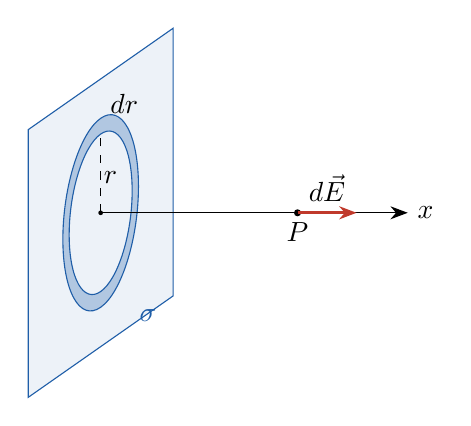
\begin{tikzpicture}[scale=1.0]
  \begin{scope}[cm={-0.4,-0.28,0,1,(0,0)}]
    \fill[azul!8] (-2.3,-1.7) rectangle (2.3,1.7);
    \draw[azul] (-2.3,-1.7) rectangle (2.3,1.7);
    \fill[azul!35, even odd rule] (0,0) circle (1.0) (0,0) circle (1.2);
    \draw[azul] (0,0) circle (1.0) (0,0) circle (1.2);
  \end{scope}
  \draw[dashed] (0,0) -- node[pos=0.45, right, inner sep=1pt]{$r$} (0,1.0);
  \node at (0.3,1.38) {$dr$};
  \draw[eje] (0,0) -- (3.9,0) node[right]{$x$};
  \fill (0,0) circle (0.03);
  \fill (2.5,0) circle (0.045) node[below]{$P$};
  \draw[->, very thick, rojo] (2.5,0) -- (3.25,0) node[above, pos=0.5, text=black]{$d\vec E$};
  \node[text=azul] at (0.6,-1.3) {$\sigma$};
\end{tikzpicture}
\end{document}
